\documentclass{article}
\usepackage[utf8]{inputenc}
\usepackage{amsmath}
\usepackage{listings}

\usepackage{amsthm}
\usepackage{graphicx}
\usepackage{upgreek}
\usepackage{algorithm}
\usepackage{algpseudocode}


\date{20 February 2019}
\marginparwidth 0.5in 
\oddsidemargin 0.25in 
\evensidemargin 0.25in 
\marginparsep 0.25in
\topmargin 0.25in 
\textwidth 6in \textheight 8 in
\newtheorem{question}{Question: }
\theoremstyle{case}
\newtheorem{case}{Case}
\graphicspath{ {images/} }
\begin{document}
\author{Sai Vineet Reddy Thatiparthi}

 \title{%
  Advanced Machine Learning \\
  \large Homework 3}
\maketitle
\begin{enumerate}
    \item [1.] \textbf{For the following figure, (a) Is A independent of C given B and D in each
of the 3 cases? (b) Is B conditionally independent of D given A and C}
\end{enumerate} 
\begin{proof} 
I will be using d-separation to figure this out.\\ \\
\textbf{(a) (i)} From the figure, we are told that $B$ and $D$ are observed. There are two paths from $A$ to $C$, which are $ABC$ and $ADC$. Let's look at the path $ABC$ - here, the figure is in a head-tail configuration, with $B$ being observed. This means that, $B$ will block the path from $A$ to $C$. The same thing happens in the other path too. Since both paths are blocked, we can conclude that $A$ is conditionally independent of $C$ given $B, D$.\\ \\
\textbf{(ii)} From the figure, $B$ and $C$ are observed. There are two paths from $A$ to $C$, which are $ABC$ and $ADC$. Let's look at the path $ABC$ - here, the figure is in a head-head configuration, where $B$ is being observed. $B$ will block the path from $A$ to $C$. In an H-H configuration, a path becomes unblocked if the node is observed. This means that $B$ will not block the path. Hence, A is dependent on C given B and D.\\ \\
\textbf{(b)(i)} From the figure, we are told that $A$ and $C$ are observed. There are two paths from $B$ to $D$, which are $DCB$ and $DAB$. Let's look at the path $DCB$ - here, the figure is in a head-head configuration. Since C is being observed, the path becomes unblocked. Hence, we can safely say that B is not independent of D given A and C. \\ \\
\textbf{(b)(ii)} From the figure, we are told that $A$ and $C$ are observed. There are two paths from $B$ to $D$, which are $DCB$ and $DAB$. Let's look at the path $DAB$ - it is in a tail-tail configuration with A being observed. This means that A will block the path from D to B. Now coming to path DCB - it it is also in a tail-tail configuration with C being observed. This means that C will block the path from D to B. Hence, since both paths are blocked, we get that D is independent of B given A and C.
\end{proof}

\begin{enumerate}
    \item [2.] \textbf{Consider the problem discussed in class (Notes set 5-bn.pdf; the example
with heat disease etc.). Infer the probability that an individual has heart
disease given that the individual has high blood pressure, has health diet
and exercise regularly}
\end{enumerate}
\begin{proof}
We need to find $P(HD = Y|BP=Y,D = H, E = Y)$. To do this, we can do the following - 
\begin{gather*}
    = \frac{P(HD, BP, D, E, CP, HB}{P(BP, D, E)}
\end{gather*}
We do this because we need to marginalise on all the unknown features too.
\begin{gather*}
    = \frac{\sum_{HB}\sum_{CP}P(E)P(D)P(HD|E,D)P(HB|E,D)P(BP|HD),P(CP|HB,|HD)}{\sum_{HB}\sum_{CP}\sum_{HD}P(E)P(D)P(HD|E,D)P(HB|E,D)P(BP|HD),P(CP|HB,|HD)}
\end{gather*}
This is the marginalisation step. \\ \\
This is the numerator
\begin{gather*}
    \alpha \sum_{HB}P(HB|D)\sum_{CP}P(CP|HB,HD)\\
    \end{gather*}
    This is the denominator
    \begin{gather*}
    \beta \sum_{HB}P(HB|D)\sum_{HD}P(BP|HD)P(HD|E,D)\sum_{CP}P(CP|HB,HD) \\
    \end{gather*}
here, $\beta = P(E)P(D)$ and $\alpha = P(E)P(D) P(HD|E,D) P(BP|HD)$ \\ \\
To simplify the summations (we look at the data), in the numerator we get = 
\begin{gather*}
= \sum_{HB}P(HB|D)\sum_{CP}P(CP|HD,HB) * \alpha\\
= 0.2 * (0.8+0.2) + 0.8(0.6+0.4) *\alpha \\ 
= 1 * \alpha \\
= 1* 0.7*0.25*0.25*0.85\\
Numerator = 0.2125
\end{gather*}
The denomintor simplifies to = 
\begin{gather*}
    = \beta * \sum_{HB}P(HB|D)\sum_{HD}P(BP|HD)P(HD|E,D)\sum_{CP}P(CP|HB,HD)\\
    = 0.85 * 0.25 (0.2(0.8+0.2)) + 0.85 * 0.25(0.8 (0.8*0.4)) + 0.2*0.75(0.2) + 0.2*0.75*0.8 \\
    Denominator = 0.3625
\end{gather*}
Now, dividing the numerator and denominator we get, 
\begin{gather*}
    \frac{0.2125}{0.3625} = 0.5862
\end{gather*}
So, $P(HD = Y|BP=Y,D = H, E = Y) = 0.5862$
\end{proof}
\begin{enumerate}
    \item [3.] \textbf{Induce the Bayesian network topology for the following problem: Two
algorithms, A1 and A2 continually observe intrusions into a computer
network. Suppose, A1 indicates an intrusion while A2 does not. Sometimes
an intrusion is detected because the system administrator upgraded a
previous version of an application. Is there an intrusion? Make as many
reasonable assumptions as required.}
\end{enumerate} 
\begin{proof} 
The features that we will assume are present and affecting our computer network are - 
\begin{itemize}
  \item OS Version = OS (Computers having old or new OS's)
  \item Auto Update = AU (Probability of an auto update)
  \item Intrusion = I (Probability of an intrusion)
  \item Algorithm A1 =  $A_1$
  \item Algorithm A2 = $A_2$
\end{itemize}
The probability joint distribution and the topology will be as follows (look at figure 1) \\ \\
\begin{figure}[h]
            \caption{Bayesian Network Topology}
            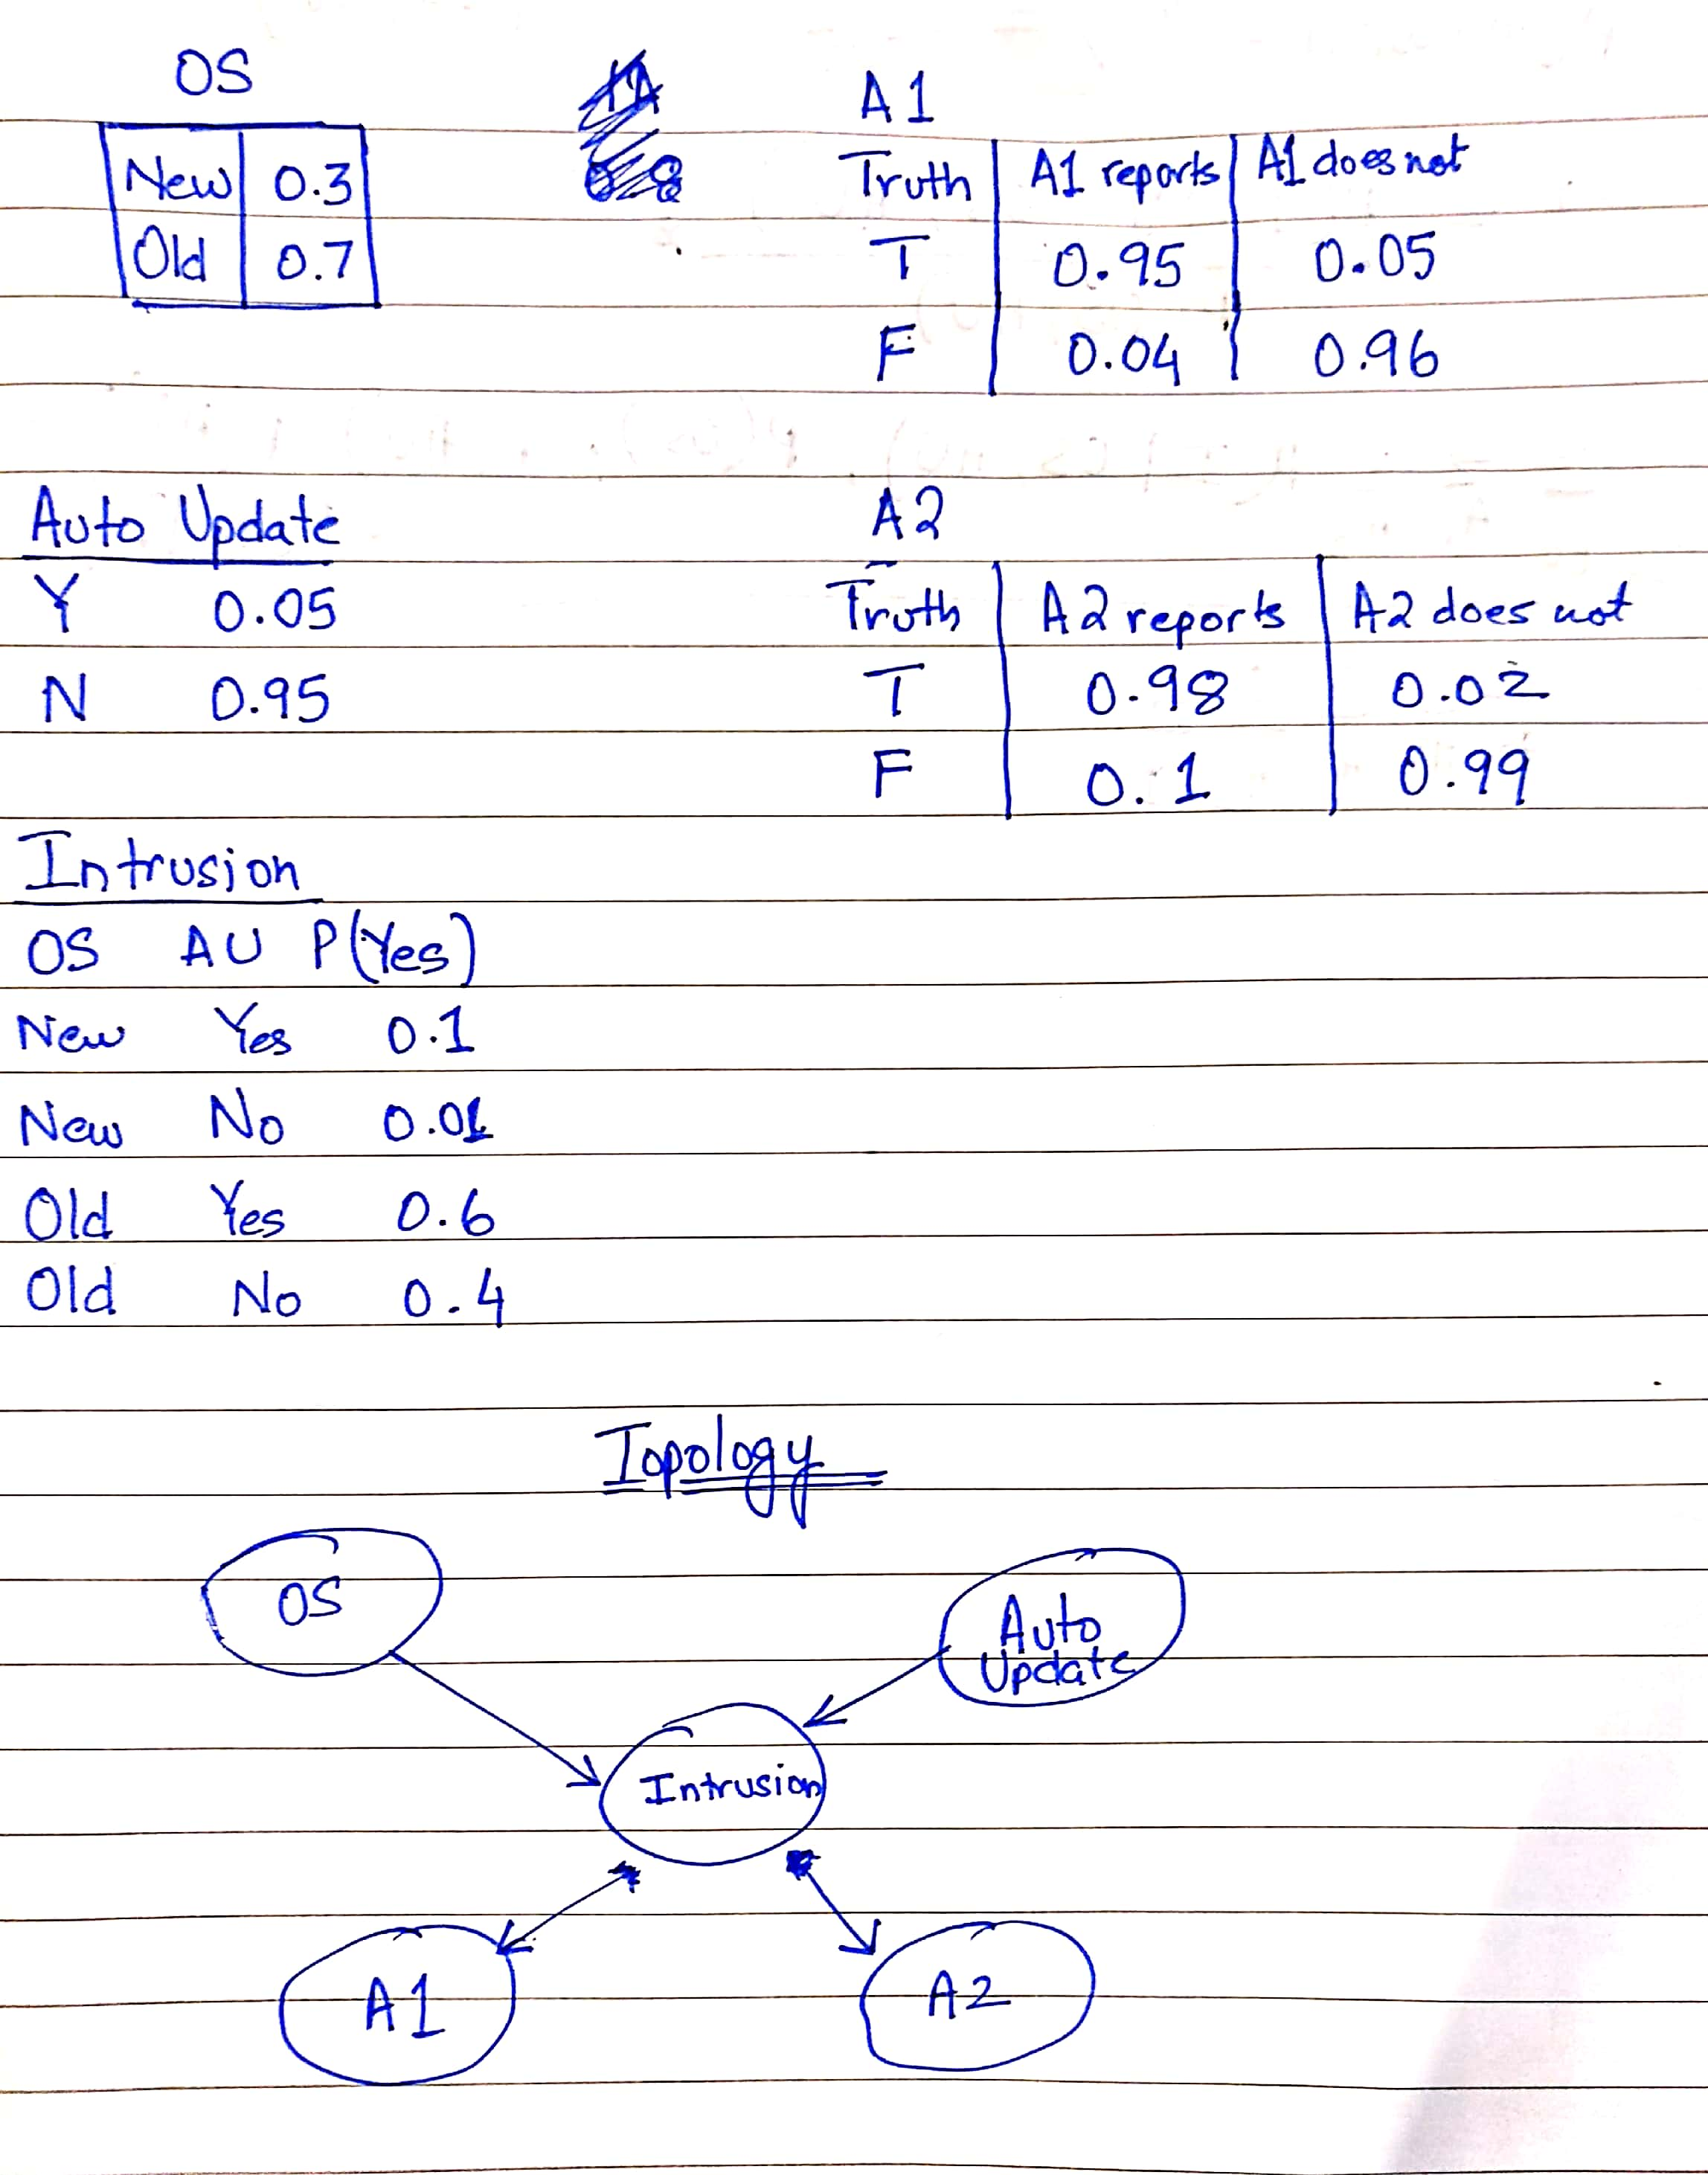
\includegraphics[scale=0.2]{img3.jpg}
            % \centering
            \end{figure}
$A_1$ and $A_2$ will be monitoring for intrusions. \\
We need to calculate  $P(Intrusion = Y)$ = \\
\begin{gather*}
    = P(I = Y|OS, AU = Y) \\
    = \frac{P(I = Y,OS,AU = Y)}{P(OS,AU)}\\
    = \frac{\sum_{OS}\sum_{A1}\sum_{A2}P(I=Y|OS,AU= Y).P(OS).P(AU=Y).P(A1|I=Y).P(A2|I=Y)}{\sum_{OS}\sum_{AU}\sum_{A1}\sum_{A2}\sum_{I}P(I|OS,AU).P(OS).P(AU).P(A1|I).P(A2|I)} \\
\end{gather*}
We take auto update = Yes because the system just finished an automatic software update. We just need to compute the probability of when an intrusion has actually occurred, hence we equate it to Y as well. This is the reason why the numerator has this conditions present and also the reason why we do not marginalise on I and AU. However, since the denominator is different, we marginalise there on all features that can vary.  \\ \\
P (Intrusion) was too cumbersome to calculate so I just left the formula the way it is above, you just have to substitute the values. We can just plug the values in from the figure 1 to compute it. After calculating this Probability, we will have the value of P(Intrusion = YES). If the probability is higher than 0.5, then we say that an intrusion actually might have occurred. If it is lower than 0.5, we say that an intrusion has not occurred. 
\end{proof}

\end{document}